% L4a student companion deck.
%
% The frame order mirrors the lecture notebook so students can take notes while
% the instructor works through the notebook. The disclaimer is intentionally
% slide 2, by instructor preference.
\documentclass[aspectratio=169,11pt]{beamer}
\usepackage{vnslides}

\newcommand{\Pmeasure}{\mathbb{P}}

\title{\texorpdfstring{{\vnheavy L4a}}{L4a}: Trading Rules Using Binomial Lattice Models}
\subtitle{CHEME 5660 Cornell University}
\author{Copyright Jeffrey Varner 2026. All Rights Reserved}

\begin{document}

\vntitlepage

\begin{frame}{Disclaimer and Risks}
  \vspace{0.6em}
  \textbf{\ink{Training only.}} This content is for training and informational
  purposes only. The teaching team does not make, give, or endorse any offer or
  solicitation to buy or sell securities or derivative products, or provide
  investment or trading advice or strategy.

  \vspace{1.1em}
  \textbf{\ink{Risk.}} Trading involves risk and is generally not recommended for
  those with limited resources, experience, or a low risk tolerance. Past
  performance does not guarantee future success.

  \vspace{1.1em}
  \textbf{\ink{Responsibility.}} You are responsible for your investment decisions
  based on your financial circumstances, objectives, risk tolerance, and
  liquidity needs.
\end{frame}

\begin{frame}{Objectives for Today}
By the end of this lecture, you will be able to:

  \vspace{0.8em}
  \begin{itemize}\setlength{\itemsep}{0.8em}
    \item \hilite{Evaluate a stock trade using NPV}: derive the scaled NPV
      and explain how sale price, holding period, and benchmark affect it.
    \item \hilite{Compute terminal target probabilities}: find the minimum
      up-move count needed to exceed a target and add the binomial probabilities.
    \item \hilite{Extend the lattice to $m$ outcomes per step}:
      use branch counts to calculate node prices, probabilities, and state counts.
  \end{itemize}
\end{frame}

\begin{frame}{Lectures and Examples}
\textbf{\ink{Lecture:}}
  \href{https://github.com/varnerlab/CHEME-5660-CourseRepository-Fall-2026/blob/main/lectures/week-4/L4a/CHEME-5660-L4a-Lecture-LatticeModel-TradeRule-Fall-2026.ipynb}{Trading Rules Using Binomial Lattice Models}

  \vspace{1.1em}
  \textbf{\ink{Example:}}
  \href{https://github.com/varnerlab/CHEME-5660-CourseRepository-Fall-2026/blob/main/lectures/week-4/L4a/CHEME-5660-L4a-Example-CumulativeProbabilityLattice-Fall-2026.ipynb}{Binomial Lattice Terminal-Target Probabilities}

  What is the probability of exceeding a target scaled NPV? We estimate the
  lattice parameters from historical data and compare probabilities across targets.

  \vspace{1.1em}
  \textbf{\ink{Example:}}
  \href{https://github.com/varnerlab/CHEME-5660-CourseRepository-Fall-2026/blob/main/lectures/week-4/L4a/CHEME-5660-L4a-Example-N-Ary-Lattice-Fall-2026.ipynb}{N-Ary Recombining Lattice Models}

  What changes when we allow more price movements per step? We estimate branch
  factors and probabilities, build the lattice, and examine its terminal outcomes.
\end{frame}

\begin{frame}{From Bid and Ask Quotes to a Lattice Price}
\href{https://www.citadelsecurities.com/who-we-are/}{Citadel Securities}
  is a \hilite{market maker}: it stands ready to buy from sellers and sell to buyers.

  \vspace{0.6em}
  At time $t$, its quotes are:
  \begin{itemize}\setlength{\itemsep}{0.4em}
    \item \hilite{Bid $b_t$}: the price at which it will buy.
    \item \hilite{Ask $a_t$}: the price at which it will sell.
  \end{itemize}

  The spread $s_t$ and midpoint $m_t$ are:
  \[
    \underbrace{s_t=a_t-b_t}_{\text{bid--ask spread}},
    \qquad
    \underbrace{m_t=\frac{a_t+b_t}{2}}_{\text{midpoint}}.
  \]

  For today's model, we replace the bid and ask with one frictionless price
  $S_t$. The lattice assigns probabilities to its possible future values.
\end{frame}

\begin{frame}{A Recombining Price Lattice}
Each step lasts $\Delta t$ years. Up and down branches multiply the price
  by $u$ and $d$; paths with the same counts reach the same node.
  \begin{center}
    
\includegraphics[width=\linewidth,height=0.66\textheight,keepaspectratio]{../figs/Fig-Lattice-Schematic.pdf}
  \end{center}
\end{frame}

\begin{frame}{The Binomial Lattice Model}
Start at price $S_0>0$. Each step multiplies the price by $u$ with real-world
  probability $p$, or by $d$ with probability $1-p$, where $u>d>0$ and $0<p<1$.

  \vspace{0.5em}
  Assume \hilite{independent moves} and fixed $(u,d,p)$. Let $t$ count steps
  and $K_t$ count up moves. Then $K_t\sim\operatorname{Binomial}(t,p)$:
  \[
    \underbrace{S_{t,k}=S_0u^kd^{t-k}}_{\text{node price}},
    \qquad
    \underbrace{\Pmeasure(K_t=k)=\binom tk p^k(1-p)^{t-k}}_{\text{node probability}},
    \quad k=0,\ldots,t.
  \]

  Each level contains $t+1$ price states. Independent moves with fixed
  parameters do not capture volatility clustering.
\end{frame}

\begin{frame}{The Trade We Will Evaluate}
Suppose we buy shares now and sell them after a chosen holding period.

  \vspace{0.7em}
  \begin{itemize}\setlength{\itemsep}{0.65em}
    \item Buy $n_0>0$ shares at price $S_0>0$ USD/share at time zero.
    \item Hold for $N$ steps of duration $\Delta t>0$ years; sell at
      $T=N\Delta t$ for $S_T$ USD/share.
    \item Discount the sale proceeds using a constant annual benchmark
      growth rate $g_y$, measured in inverse years.
  \end{itemize}

  \vspace{0.6em}
  We assume no dividends, transaction fees, or bid--ask spread.
\end{frame}

\begin{frame}{Net Present Value of a Long Position}
Use the continuously compounded benchmark $g_y$ for yield $y$: a risk-free
  rate or an assumed growth rate for another investment. The trade's NPV is:
  \[
    \underbrace{\operatorname{NPV}(g_y,T)}_{\text{time-0 dollars}}
    =\underbrace{-n_0S_0}_{\text{purchase today}}
    +\underbrace{n_0S_Te^{-g_yT}}_{\text{discounted sale proceeds}}.
  \]

  Divide by the initial investment to obtain the dimensionless scaled NPV:
  \[
    \underbrace{\rho_T}_{\text{scaled NPV}}
    :=\frac{\operatorname{NPV}(g_y,T)}{n_0S_0}
    =e^{-g_yT}\frac{S_T}{S_0}-1.
  \]

  If $\rho_T>0$, the discounted sale proceeds exceed the purchase cost.
  Scaling removes the dependence on the number of shares.
\end{frame}

\begin{frame}{Sale Price and Discounted NPV}
\begin{center}
    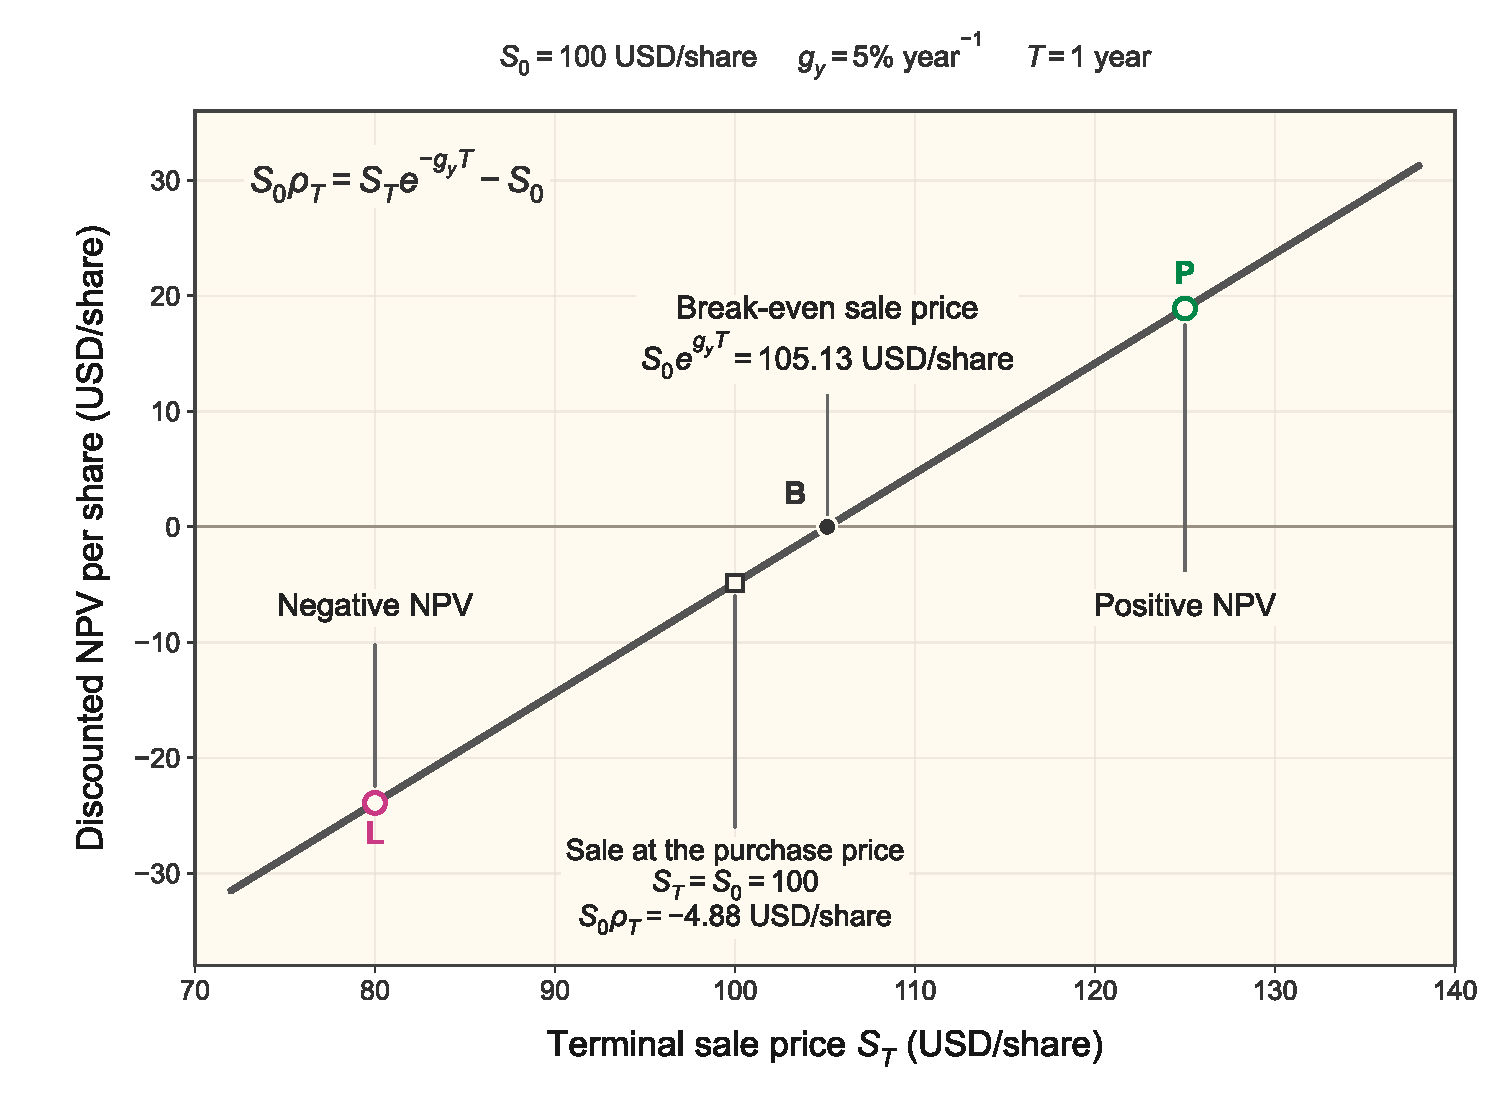
\includegraphics[width=0.96\linewidth,height=0.79\textheight,keepaspectratio]{../figs/Fig-TradeRule-Schematic.pdf}
  \end{center}
\end{frame}

\begin{frame}{Short Holding Periods}
When $|g_y|T\ll1$, the discount factor $e^{-g_yT}$ is close to one.
  The scaled NPV is approximately the fractional change in share price:
  \[
    \underbrace{\rho_T}_{\text{scaled NPV}}
    \approx \underbrace{\frac{S_T}{S_0}-1}_{\text{price return}}.
  \]

  \vspace{0.7em}
  Buying at 100 USD/share and selling at 105 USD/share gives:
  \[
    \frac{105}{100}-1=0.05=5\%.
  \]
  When discounting has little effect, the scaled NPV is approximately 5\%.
\end{frame}

\begin{frame}{Longer Holding Periods}
As the holding period grows, discounting can have a substantial effect.
  The sale price that makes the scaled NPV zero satisfies:
  \[
    e^{-g_yT}\frac{S_T}{S_0}-1=0
    \quad\Longrightarrow\quad
    \underbrace{S_T=S_0e^{g_yT}}_{\text{break-even sale price}}.
  \]

  For $g_y>0$, a positive NPV requires the sale price to exceed the purchase
  price grown at the benchmark rate.

  \vspace{0.7em}
  We use the exact discounted expression for all holding periods.
  Each lattice price gives a scaled NPV with the same probability.
\end{frame}

\begin{frame}{Terminal Target Probability}
At the scheduled sale time $T=N\Delta t$, we calculate the probability
  that the scaled NPV exceeds a chosen target $\rho_\star$:
  \[
    \Pmeasure(\rho_T>\rho_\star).
  \]

  A target $\rho_\star=0.05$ means that the discounted sale proceeds must
  exceed the initial investment by more than 5\%. Equality does not count.

  \vspace{0.7em}
  We identify terminal nodes whose scaled NPV exceeds the target and add their
  probabilities. Each terminal price is determined by the number of up moves.
\end{frame}

\begin{frame}{From Up Moves to Scaled NPV}
The up-move count is $K_N\sim\operatorname{Binomial}(N,p)$.
  A terminal node with $k$ up moves has:
  \[
    S_T=S_0u^kd^{N-k},\qquad k=0,\ldots,N.
  \]
  Substituting into the scaled NPV gives:
  \[
    \rho(k)=u^kd^{N-k}e^{-g_yN\Delta t}-1,
    \qquad \rho_T=\rho(K_N).
  \]

  Increasing $k$ replaces a down factor $d$ with an up factor $u$.
  Since $u/d>1$, both the price and scaled NPV increase.

  \vspace{0.5em}
  Once a node's scaled NPV exceeds the target, every larger up-move count succeeds.
\end{frame}

\begin{frame}{Finding the Up-Move Threshold}
For $\rho_\star>-1$, start with the strict target at a node with $k$ up moves:
  \[
    e^{-g_yN\Delta t}u^kd^{N-k}-1>\rho_\star.
  \]
  Add one, remove the discount factor, and take natural logarithms:
  \[
    k\ln(u/d)>\ln(1+\rho_\star)+g_yN\Delta t-N\ln d.
  \]
  Since $\ln(u/d)>0$, the condition becomes $k>\tau(\rho_\star)$, where:
  \[
    \underbrace{\tau(\rho_\star)}_{\text{up-move threshold}}
    =\frac{\ln(1+\rho_\star)+g_yN\Delta t-N\ln d}{\ln(u/d)}.
  \]
\end{frame}

\begin{frame}{Strict Targets Need the Next Integer}
We need $K_N>\tau(\rho_\star)$. Since the up-move count is an integer,
  the smallest integer strictly above the threshold is:
  \[
    \kappa=\lfloor\tau(\rho_\star)\rfloor+1.
  \]
  Here, $\lfloor x\rfloor$ is the greatest integer less than or equal to $x$.

  \vspace{0.7em}
  \begin{itemize}\setlength{\itemsep}{0.7em}
    \item If $\tau=2.4$, we need at least three up moves.
    \item If $\tau=2$ exactly, we still need three. Two would only
      reach the target.
  \end{itemize}
\end{frame}

\begin{frame}{Example: A Three-Month Trade}
Hold for $N=3$ monthly steps: $\Delta t=1/12$ year and $T=1/4$ year.
  Use $u=1.10$, $d=0.90$, $p=0.6$, and $g_y=0.04\,\mathrm{year}^{-1}$.

  \vspace{0.5em}
  To exceed a target scaled NPV of 5\%, the up-move threshold is:
  \[
    \tau(0.05)
    =\frac{\ln(1.05)+0.04(3/12)-3\ln(0.90)}{\ln(1.10/0.90)}
    \approx1.868.
  \]
  We need at least $\kappa=2$ up moves. Check the two neighboring returns:
  \[
    \rho(1)\approx-0.1179,\qquad \rho(2)\approx0.0782.
  \]
  Two up moves exceed the 5\% target; one does not.
\end{frame}

\begin{frame}{Example: Add Successful Node Probabilities}
The successful counts in the three-month trade are $K_3=2$ and $K_3=3$.
  With $p=0.6$, their combined probability is:
  \[
    \begin{aligned}
      \Pmeasure(\rho_T>0.05)
      &=\Pmeasure(K_3\ge2)\\[0.3em]
      &=\binom32(0.6)^2(0.4)+\binom33(0.6)^3\\[0.3em]
      &=0.432+0.216=0.648.
    \end{aligned}
  \]

  The model assigns a \hilite{64.8\% probability} to exceeding the target
  at the scheduled sale time.

  \vspace{0.5em}
  The return inequality determines which counts succeed.
  The probability $p$ determines how much probability those counts carry.
\end{frame}

\begin{frame}{Computing the Cumulative Probability}
The up-move count ranges from $0$ to $N$. Record the cutoff as:
  \[
    k_{\min}=\min\!\left\{\max\!\left\{\kappa,0\right\},N+1\right\}.
  \]
  For $\rho_\star>-1$, add the probabilities of the successful counts:
  \[
    \Pmeasure(\rho_T>\rho_\star)=
    \begin{cases}
      1, & k_{\min}=0\quad\text{(all nodes)},\\[0.35em]
      \displaystyle\sum_{k=k_{\min}}^N\binom Nk p^k(1-p)^{N-k},
        & 1\le k_{\min}\le N,\\[0.35em]
      0, & k_{\min}=N+1\quad\text{(no nodes)}.
    \end{cases}
  \]

  The sum is the \hilite{binomial upper tail}. For $\rho_\star\le-1$,
  the probability is one because every model price is positive.
\end{frame}

\begin{frame}{What About Falling Short of the Target?}
At the scheduled sale time, the scaled NPV either exceeds the target or
  finishes at or below it. These events are complementary:
  \[
    \Pmeasure(\rho_T\le\rho_\star)=1-\Pmeasure(\rho_T>\rho_\star).
  \]
  For $\rho_\star=-0.05$, this gives the probability that the discounted
  fractional return finishes at or below $-5\%$.

  \vspace{0.6em}
  Increasing $g_y$ with the lattice and target fixed cannot increase the success
  probability. Changing $N$ changes both the cutoff and the count distribution.

  \slidenote{Scheduled sale:}{this calculation checks the final outcome. Selling when a boundary is first reached requires the price path; see the optional first-passage example.}
\end{frame}

\begin{frame}{Example: Terminal Targets from Data}
\textbf{\ink{Example:}}
  \href{https://github.com/varnerlab/CHEME-5660-CourseRepository-Fall-2026/blob/main/lectures/week-4/L4a/CHEME-5660-L4a-Example-CumulativeProbabilityLattice-Fall-2026.ipynb}{Explore a terminal target probability}

  \vspace{0.7em}
  How likely are we to exceed our target when we fit the lattice to historical data?

  \vspace{0.5em}
  \begin{itemize}\setlength{\itemsep}{0.6em}
    \item Estimate the up and down factors and up-move probability.
    \item Identify terminal nodes whose scaled NPV exceeds the target.
    \item Add their probabilities and compute the complement.
  \end{itemize}

  \slidenote{Next question:}{what changes if each step allows more than two price movements?}
\end{frame}

\begin{frame}{A Three-Outcome Price Model}
An N-ary lattice allows $m$ outcomes per step. Suppose $S_0=100$ USD/share.
  With $m=3$, the price can increase by 10\%,
  remain unchanged, or decrease by 10\%.

  \vspace{0.6em}
  \begin{center}
    \renewcommand{\arraystretch}{1.3}
    \begin{tabular}{lrrr}
      \toprule
      Movement & Factor $f_j$ & Probability $p_j$ & Price after one step\\
      \midrule
      Up 10\% & 1.10 & 0.25 & 110\\
      Unchanged & 1.00 & 0.50 & 100\\
      Down 10\% & 0.90 & 0.25 & 90\\
      \bottomrule
    \end{tabular}
  \end{center}

  \vspace{0.5em}
  Up then down gives $100(1.10)(0.90)=99$ USD/share. Reversing the order gives
  the same price. Both have counts $(1,0,1)$ for up, unchanged, and down moves, so they share one node.
\end{frame}

\begin{frame}{Computing an N-Ary Node's Price}
Allow $m\ge2$ branches with fixed price factors $f_j>0$ and probabilities
  $p_j>0$, where $\sum_{j=1}^mp_j=1$. At level $t$, let $x_j$ count branch $j$:
  \[
    \mathbf{x}=(x_1,\ldots,x_m),\qquad
    x_j\in\mathbb{Z}_{\ge0},\qquad \sum_{j=1}^mx_j=t.
  \]
  Each occurrence of branch $j$ multiplies the price by $f_j$:
  \[
    \underbrace{S_t(\mathbf{x})}_{\text{node price}}
    =S_0\prod_{j=1}^mf_j^{x_j}.
  \]
  For our three-outcome model, $S_2(1,0,1)=100(1.10)(0.90)=99$ USD/share.
  The counts determine the final price; the order can change intermediate prices.
\end{frame}

\begin{frame}{Computing an N-Ary Node's Probability}
Assume independent branch choices with fixed probabilities.
  Let $\mathbf{X}_t$ be the random vector of branch counts after $t$ steps.

  \vspace{0.5em}
  Up--down and down--up each have probability $0.25^2=0.0625$.
  Both reach $(1,0,1)$, so this node has probability $0.125$.

  \vspace{0.5em}
  In general, add the probabilities of all paths with the same counts:
  \[
    \Pmeasure(\mathbf{X}_t=\mathbf{x})
    =\underbrace{\frac{t!}{x_1!\cdots x_m!}}_{\text{number of orderings}}
     \underbrace{\prod_{j=1}^mp_j^{x_j}}_{\text{probability of one ordering}}.
  \]
  With $m=2$, this reduces to the binomial probability
  $\binom tk p^k(1-p)^{t-k}$.
\end{frame}

\begin{frame}{Nine Paths Recombine into Six Count States}
After two steps, there are $3^2=9$ ordered paths. We only need six count states:

  \vspace{0.35em}
  \begin{center}
    \renewcommand{\arraystretch}{1.18}
    \begin{tabular}{crrr}
      \toprule
      Counts (up, unchanged, down) & Paths & Price (USD/share) & Probability\\
      \midrule
      $(2,0,0)$ & 1 & 121 & 0.0625\\
      $(1,1,0)$ & 2 & 110 & 0.2500\\
      $(1,0,1)$ & 2 & 99 & 0.1250\\
      $(0,2,0)$ & 1 & 100 & 0.2500\\
      $(0,1,1)$ & 2 & 90 & 0.2500\\
      $(0,0,2)$ & 1 & 81 & 0.0625\\
      \bottomrule
    \end{tabular}
  \end{center}

  The six probabilities sum to one and give the two-step price distribution.
\end{frame}

\begin{frame}{Example: A Target in the Three-Outcome Model}
Use the preceding table with $S_0=100$ USD/share, $N=2$ monthly steps,
  $T=1/6$ year, and $g_y=0.04\,\mathrm{year}^{-1}$.

  \vspace{0.5em}
  A target scaled NPV of 5\% requires:
  \[
    S_T>S_0(1+\rho_\star)e^{g_yT}
    =100(1.05)e^{0.04/6}\approx105.70\text{ USD/share}.
  \]
  Only $(2,0,0)$ and $(1,1,0)$, priced at 121 and 110 USD/share, qualify.
  Add their probabilities:
  \[
    \Pmeasure(\rho_T>0.05)=0.0625+0.2500=0.3125.
  \]
  The model assigns a \hilite{31.25\% probability} to exceeding the 5\% target
  at the scheduled sale time, two months after purchase.
\end{frame}

\begin{frame}{How Many States Do We Need?}
A count state satisfies $x_1+\cdots+x_m=t$. Represent the $t$ moves by stars
  and separate the $m$ branch groups using $m-1$ bars:
  \[
    \star\;|\;|\;\star\quad\longleftrightarrow\quad(1,0,1).
  \]

  Choose the bar positions among $t+m-1$ available positions:
  \[
    L_t=\binom{t+m-1}{m-1},
    \qquad L_2=\binom42=6\quad\text{when }m=3.
  \]

  This counts branch-count states, not necessarily distinct prices. If
  $f_1f_3=f_2^2$, for example, $(1,0,1)$ and $(0,2,0)$ share a price.
  We add their probabilities when computing the probability of that price.
\end{frame}

\begin{frame}{Example: N-Ary Lattices from Data}
\textbf{\ink{Example:}}
  \href{https://github.com/varnerlab/CHEME-5660-CourseRepository-Fall-2026/blob/main/lectures/week-4/L4a/CHEME-5660-L4a-Example-N-Ary-Lattice-Fall-2026.ipynb}{Explore N-ary lattice models}

  \vspace{0.7em}
  How do we build a lattice with several branches from historical data?

  \vspace{0.5em}
  \begin{itemize}\setlength{\itemsep}{0.6em}
    \item Estimate branch factors and probabilities from historical growth rates.
    \item Build the lattice and calculate node prices and multinomial probabilities.
    \item Check that probabilities sum to one and plot the resulting distributions.
  \end{itemize}

  \slidenote{Toward continuous time:}{lattices can approach continuous-time price models when price changes are scaled as the time step shrinks.}
\end{frame}

\begin{frame}{Optional Advanced Material}
\textbf{\ink{Advanced:}}
  \href{https://github.com/varnerlab/CHEME-5660-CourseRepository-Fall-2026/blob/main/lectures/week-4/L4a/advanced/first-passage/CHEME-5660-L4a-Advanced-FirstPassage-ExitRules-Fall-2026.ipynb}{First-Passage Exit Rules}

  What changes if we check the price after every step? We track positions until
  a take-profit or stop-loss boundary is first reached, then compare with
  checking only the final price.

  \vspace{1.0em}
  \textbf{\ink{Advanced:}}
  \href{https://github.com/varnerlab/CHEME-5660-CourseRepository-Fall-2026/blob/main/lectures/week-4/L4a/advanced/execution/CHEME-5660-L4a-Advanced-ExecutionAware-ProbabilityOfProfit-Fall-2026.ipynb}{Execution-Aware Probability of Profit}

  How do trading costs change the target probability? We include the bid--ask
  spread, fees, and unfavorable execution prices (slippage), then compare
  the result with the frictionless calculation.

  \vspace{0.8em}
  \dimmed{Optional; neither notebook is a prerequisite for L4b.}
\end{frame}

\begin{frame}{Summary}
We used net present value and lattice probabilities to evaluate a long stock position.

  \vspace{0.7em}
  {\large\textbf{\ink{Key takeaways}}}
  \vspace{0.3em}
  \begin{itemize}\setlength{\itemsep}{0.55em}
    \item \hilite{NPV-based trading framework}: We scaled the NPV by the initial
      investment to compare discounted sale proceeds with the purchase cost.
    \item \hilite{Terminal target probabilities}: We found the minimum up-move
      count needed to exceed a target scaled NPV, then added the successful
      node probabilities. The complement gives the probability of finishing
      at or below the target.
    \item \hilite{N-ary lattice models}: We used branch counts to calculate
      prices, multinomial probabilities, and state counts for $m$ outcomes per
      step. More branches increase the computational cost.
  \end{itemize}

  \vspace{0.5em}
  Next time: continuous-time stochastic price models.
\end{frame}

\transitionframe{Next time: continuous-time stochastic price models.}

\end{document}
